\subsection{Overview of contribution intensity}

Figure~\ref{fig:prop_traj} shows mean contribution intensity by institution across thirty rounds.
Average intensity over the run is 0.293, with median 0.092 (Table~\ref{tab:coop_summary}).
Means for SI and SFI are nearly identical (0.291 versus 0.296).
Medians diverge (0.194 versus 0.034), reflecting a thicker left tail among developing agents in SFI.
Group-mean lag-1 autocorrelation is only 0.031.
Agent-level autocorrelation is 0.215.
Average cooperation is therefore moderately positive, while path stability is limited.

\begin{table}[t]
\centering
\caption{Cooperation and inequality across two independent full-protocol seeds
(780 agent-rounds each).}
\label{tab:coop_summary}
\scriptsize
\setlength{\tabcolsep}{3pt}
\begin{tabular}{lcc}
\toprule
Statistic & Seed~1 & Seed~2 \\
\midrule
Mean intensity (all) & 0.293 & 0.365 \\
SI / SFI mean intensity & 0.291 / 0.296 & 0.364 / 0.366 \\
SI / SFI median intensity & 0.194 / 0.034 & 0.205 / 0.179 \\
SI / SFI zero share & 6.4\% / 16.2\% & 11.1\% / 22.4\% \\
Agent-mean MW $p$ (SI vs SFI) & 0.817 & 0.777 \\
Final wealth gap (dev.\ $-$ developing) & $2.15\times10^{8}$ & $5.83\times10^{8}$ \\
Final LDF pool & $4.34\times10^{9}$ & $1.30\times10^{10}$ \\
Shock coverage (R5, R10) & 0.768 & 0.768 \\
Mann--Kendall trend on round means & NS & NS \\
\bottomrule
\end{tabular}
\end{table}


\begin{figure}[t]
\centering
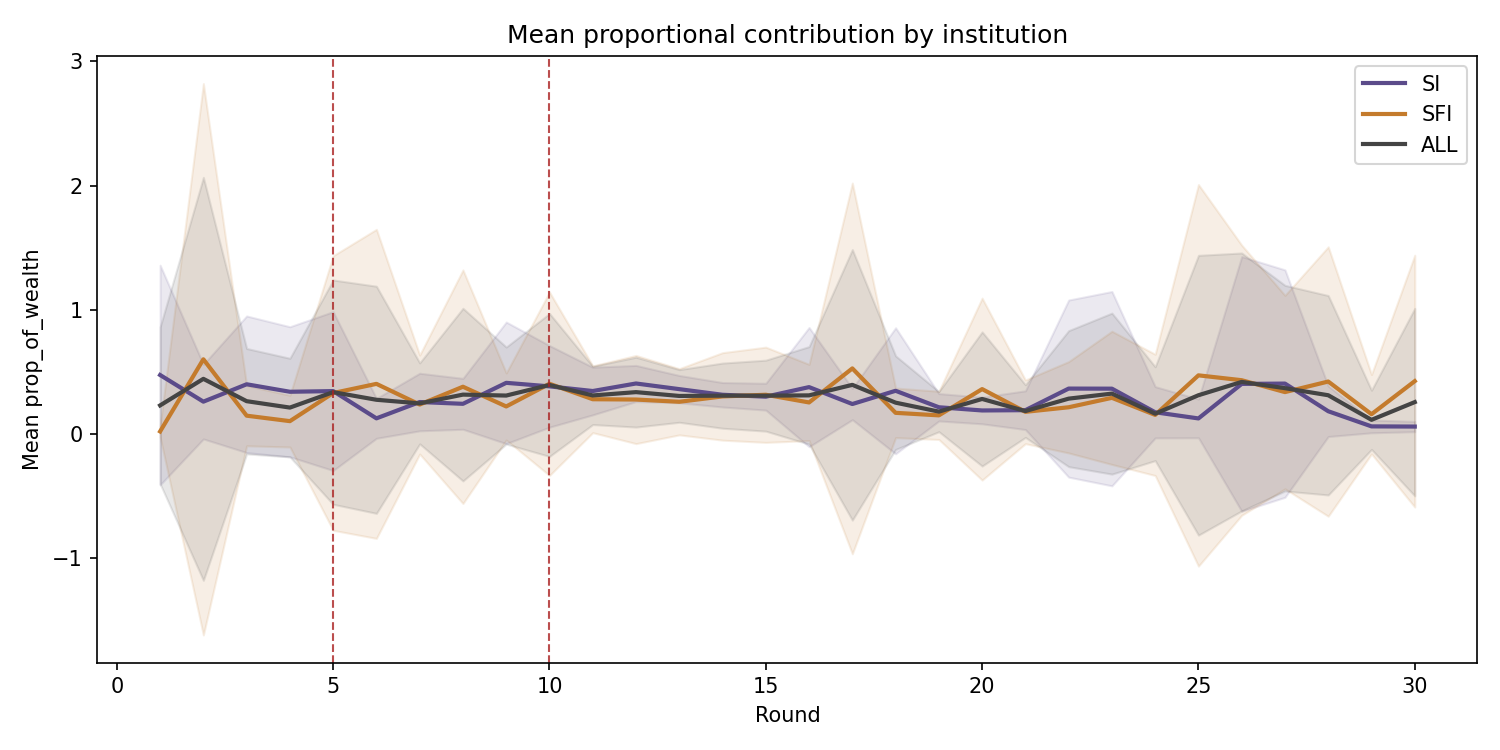
\includegraphics[width=\linewidth]{figures/contrib_mean_prop_trajectories.png}
\caption{Mean contribution intensity by institution over rounds.
Early levels are low, then rise sharply once peer history accumulates.
Institution means remain close thereafter despite forced assignment.}
\label{fig:prop_traj}
\end{figure}

Figure~\ref{fig:prop_median} reports medians with interquartile ranges.
SFI medians remain near the floor for long stretches even when means are moderate.
The distribution is right-skewed.
A minority of high-intensity rounds pulls the mean above the median.
Figure~\ref{fig:zeros} shows zero-contribution frequencies.
In round~1, 71.4\% of SFI agents contribute nothing.
Cold-start caution is common in rationales.
By round~2, SFI mean intensity jumps from 0.022 to 0.602 as peer history appears.
That spike raises average cooperation without proving an internalized contribution norm.

\begin{figure}[t]
\centering
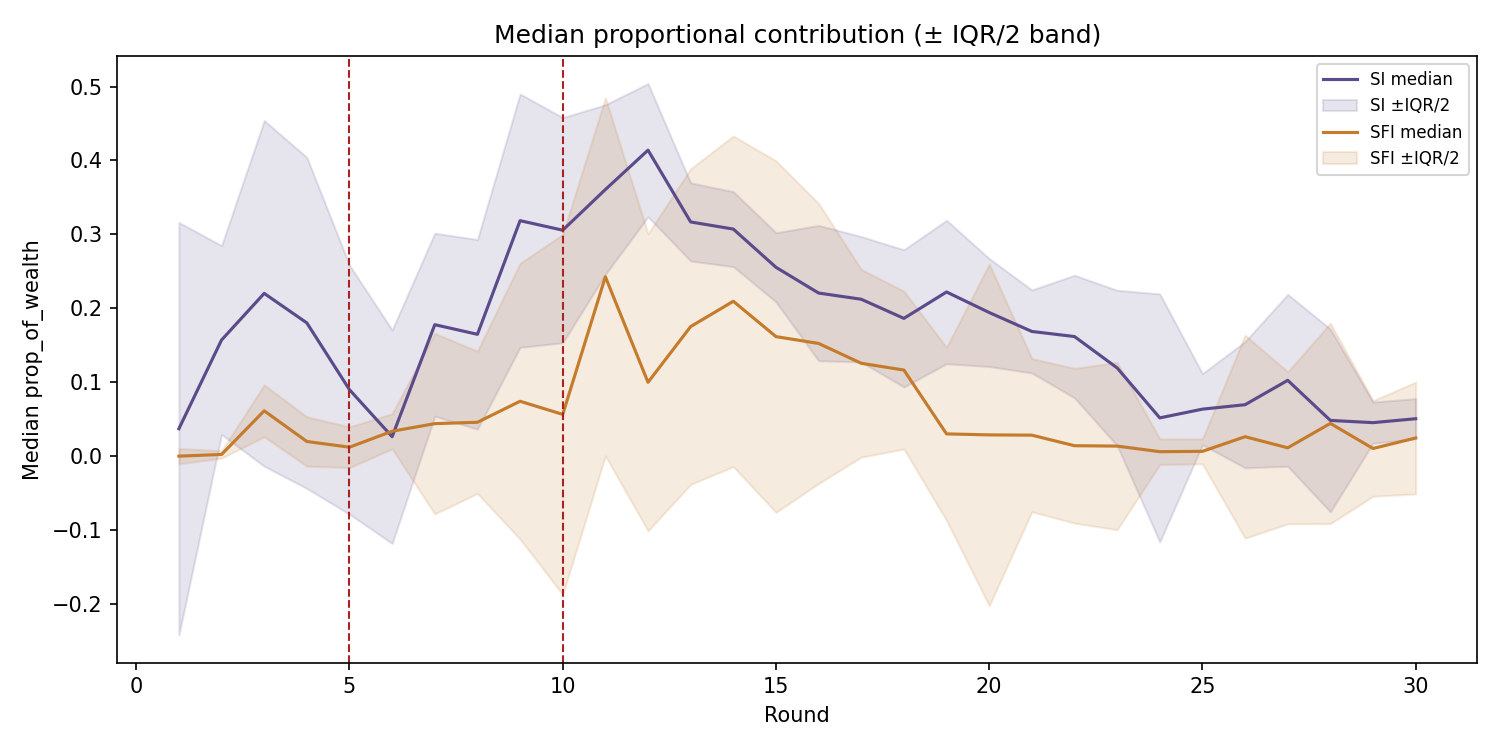
\includegraphics[width=\linewidth]{figures/contrib_median_prop_iqr.png}
\caption{Median contribution intensity with interquartile bands.
SFI medians stay low relative to means, indicating skew and fragile central tendency.}
\label{fig:prop_median}
\end{figure}

\begin{figure}[t]
\centering
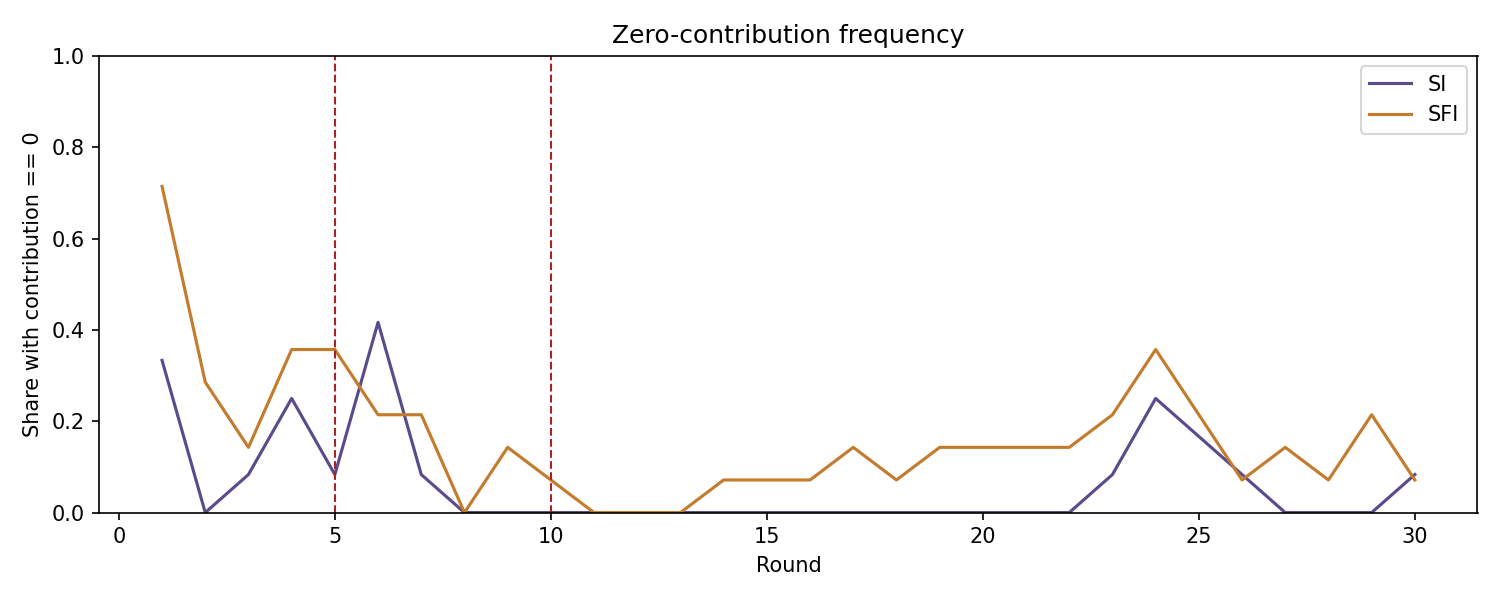
\includegraphics[width=\linewidth]{figures/contrib_zero_frequency.png}
\caption{Share of agents contributing zero by institution and round.
SFI opens with widespread zeros.
SI shows a sharp zero spike after the first climatic shock.}
\label{fig:zeros}
\end{figure}

\subsection{Main result: social pressure and subsequent intensity}

Figure~\ref{fig:rep_deltas} and Table~\ref{tab:event_study} present the primary event study.
After bad-reputation events, mean immediate $\Delta\mathrm{prop}$ is $-0.036$ in SI ($n=36$) and $-0.103$ in SFI ($n=68$).
After reputation drops, means are $-0.091$ (SI, $n=74$) and $-0.119$ (SFI, $n=81$).
After gossip targeting, means are $-0.048$ (SI, $n=35$) and $-0.201$ (SFI, $n=52$).
In every cell, fewer than two-fifths of events show a positive change.
The modal response is decline or non-increase.

\begin{figure}[t]
\centering
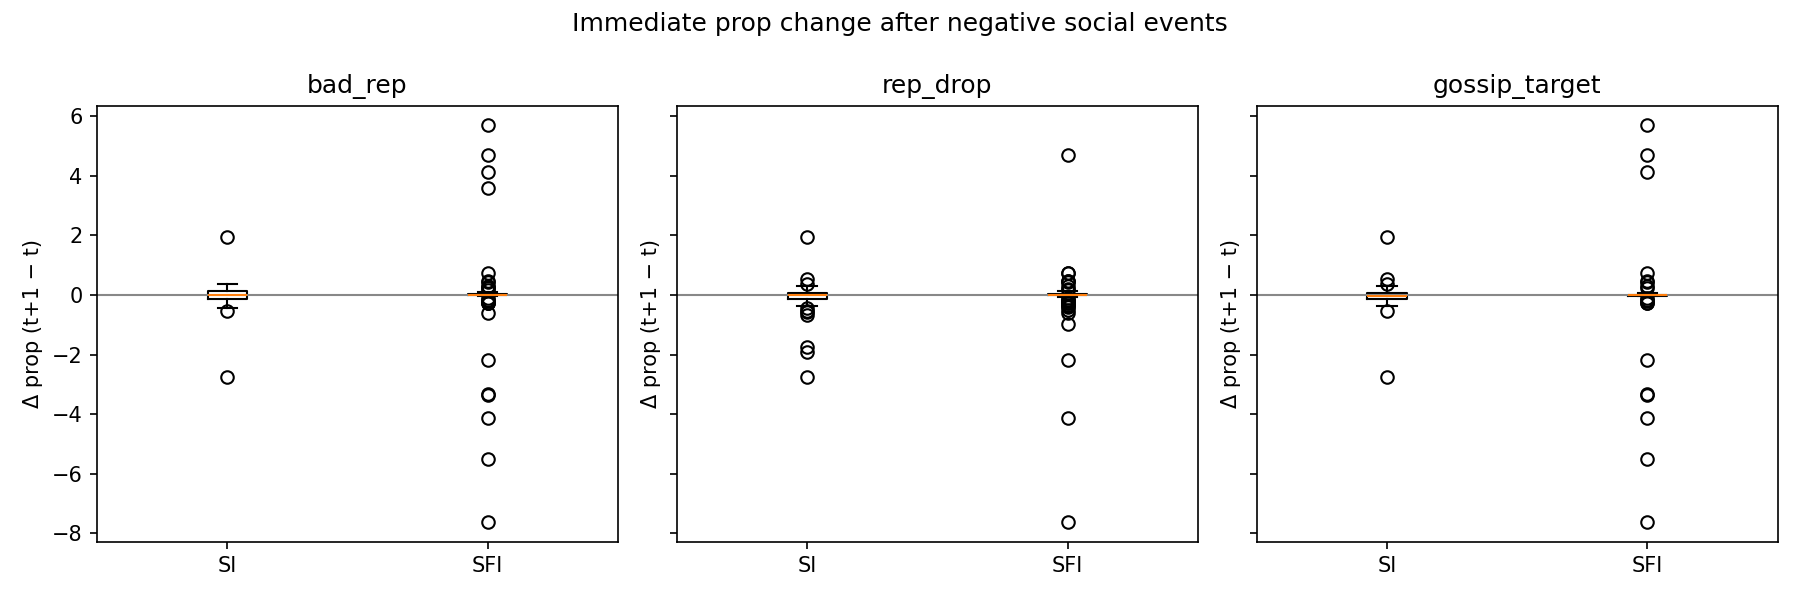
\includegraphics[width=\linewidth]{figures/reputation_event_deltas.png}
\caption{Distribution of immediate $\Delta\mathrm{prop}$ after bad-reputation, reputation-drop, and gossip-target events.
Mass lies below zero, especially for gossip targets in the non-enforcing institution.}
\label{fig:rep_deltas}
\end{figure}

\begin{table}[t]
\centering
\caption{Immediate mean $\Delta\mathrm{prop}$ after social-information events by seed and institution.
Negative cells indicate average withdrawal after the mark.}
\label{tab:event_study}
\scriptsize
\setlength{\tabcolsep}{2.8pt}
\begin{tabular}{llrr}
\toprule
Event & Inst. & Seed~1 & Seed~2 \\
\midrule
Bad reputation & SI & $-0.036$ & $+0.055$ \\
Bad reputation & SFI & $-0.103$ & $-0.069$ \\
Reputation drop & SI & $-0.091$ & $+0.058$ \\
Reputation drop & SFI & $-0.119$ & $-0.017$ \\
Gossip target & SI & $-0.048$ & $+0.187$ \\
Gossip target & SFI & $-0.201$ & $-0.084$ \\
\bottomrule
\end{tabular}
\end{table}


Gossip targets are often high contributors at the hit.
SFI gossip targets move from mean intensity 0.632 at the event to 0.430 afterward.
Overall gossip targets move from roughly 0.52 to 0.38.
Social marks therefore land on relatively visible contributors and precede lower intensity.

Table~\ref{tab:did} compares affected agents with same-round co-institution controls.
Diff-in-diff estimates are $-0.288$ for bad reputation, $-0.208$ for gossip, and $-0.143$ for reputation drops.
Controls show near-zero or slightly positive mean changes.
The association is concentrated among marked agents rather than a global round effect.

\begin{table}[t]
\centering
\caption{Diff-in-diff of $\Delta\mathrm{prop}$ versus same-round co-institution controls.}
\label{tab:did}
\scriptsize
\begin{tabular}{lccc}
\toprule
Event & Affected $\Delta$ & Control $\Delta$ & Diff-in-diff \\
\midrule
Bad reputation & $-0.291$ & $-0.003$ & $-0.288$ \\
Gossip target & $-0.197$ & $+0.011$ & $-0.208$ \\
Reputation drop & $-0.124$ & $+0.019$ & $-0.143$ \\
\bottomrule
\end{tabular}
\end{table}


First events produce larger declines than repeats.
Mean first $\Delta\mathrm{prop}$ is $-0.166$ for bad reputation, $-0.206$ for gossip, and $-0.255$ for reputation drops.
Repeat means are $-0.066$, $-0.097$, and $-0.080$, respectively.
Habituation attenuates the response without reversing the sign.

Figure~\ref{fig:gossip_freq} shows that gossip naming is concentrated rather than uniform.
A small set of agents accounts for many bulletin appearances.
Concentration is consistent with thresholded scoring in a population where most pairwise scores are low.
About 84\% of consistency scores are at most seven, so gossip eligibility is ambient.
The event study still conditions on reconstructed targeting rather than on every low score.

\begin{figure}[t]
\centering
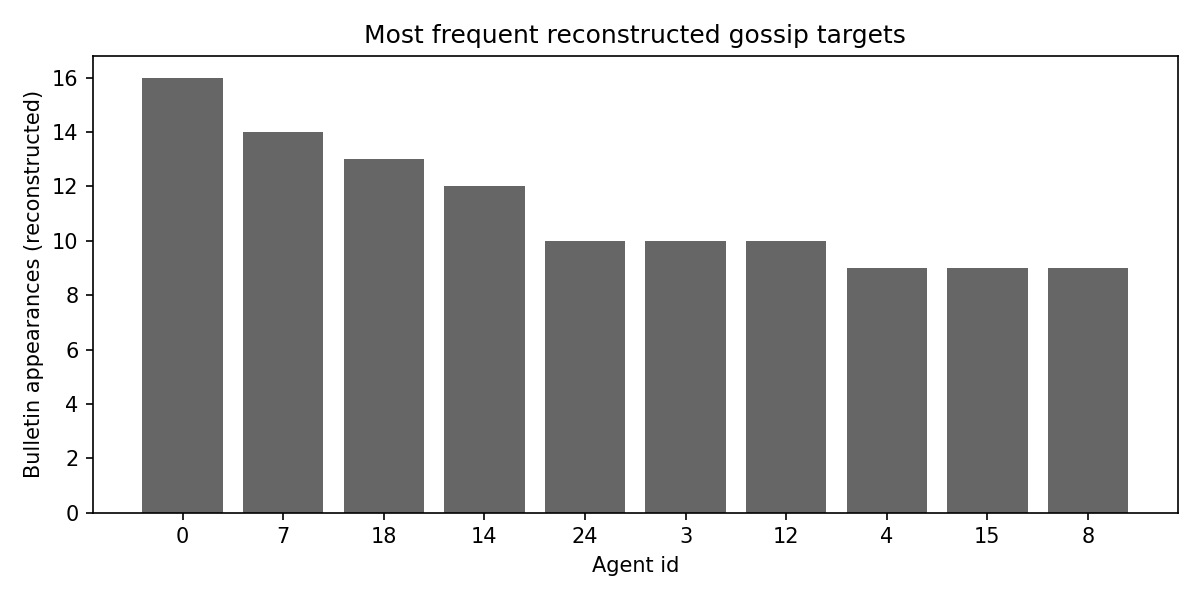
\includegraphics[width=\linewidth]{figures/gossip_target_frequency.png}
\caption{Frequency of reconstructed gossip targeting across agents.
Naming is uneven, with a subset of agents repeatedly surfacing in social bulletins.}
\label{fig:gossip_freq}
\end{figure}

\subsection{Rationales after social events}

Table~\ref{tab:motifs} summarizes coded motifs in post-event contribution texts.
Opportunistic framing appears 29 times.
Reputation-management language appears 3 times.
Conformity appears 5 times.
Explicit gossip references appear 0 times in the coded sample.
Agents seldom say they will restore standing by giving more.
They more often cite weak marginal returns and high peer contributions as reasons to give less.

\begin{table}[t]
\centering
\caption{Motifs in contribution rationales after bad-reputation or gossip events
(multi-label tag counts; $N{=}114$ post-event contribution texts).
Inter-coder reliability on a stratified 41\% subsample ($n{=}47$):
percent agreement $0.83$; Cohen's $\kappa{=}0.72$ (primary label),
$\kappa{=}0.91$ (opportunistic vs other).}
\label{tab:motifs}
\scriptsize
\begin{tabular}{lr}
\toprule
Motif & Count \\
\midrule
Opportunistic / payoff-maximizing & 29 \\
Conformity & 5 \\
Reputation management / repair & 3 \\
Named peer references & 3 \\
Future-round planning & 1 \\
Explicit gossip reference & 0 \\
\bottomrule
\end{tabular}
\end{table}


Illustrative paraphrases match the counts.
One SFI agent, after observing high peer giving, chooses zero to conserve resources and free-ride.
Another SI agent after the first shock selects zero under a high-budget, low-marginal-return logic.
A late-round SFI rationale seeks the minimum contribution that avoids a free-rider label.
That last case is reputation-aware.
It aims at a floor rather than at repair-driven escalation.
Credibility language exists as a minority pocket.
It does not dominate the motif distribution.

\subsection{Shocks, zeros, and recovery}

Figure~\ref{fig:shock_box} summarizes within-agent intensity changes around climatic shocks.
After round~5 (severity 0.10), SI mean within-agent change is $-0.178$ ($n=12$).
SFI mean change is $+0.195$ ($n=14$).
SI zero share in round~6 reaches 41.7\% (5 of 12 agents).
Many SI rationales invoke marginal-return logic after wealth and group-size updates.
After round~10 (severity 0.20), SI change is $+0.049$ and SFI change is $-0.022$.
Mean intensity during the second shock round is comparatively high (0.396).
Pre-shock mean intensity is regained in one round after the first shock and in two rounds after the second.
Permanent collapse is not observed.

\begin{figure}[t]
\centering
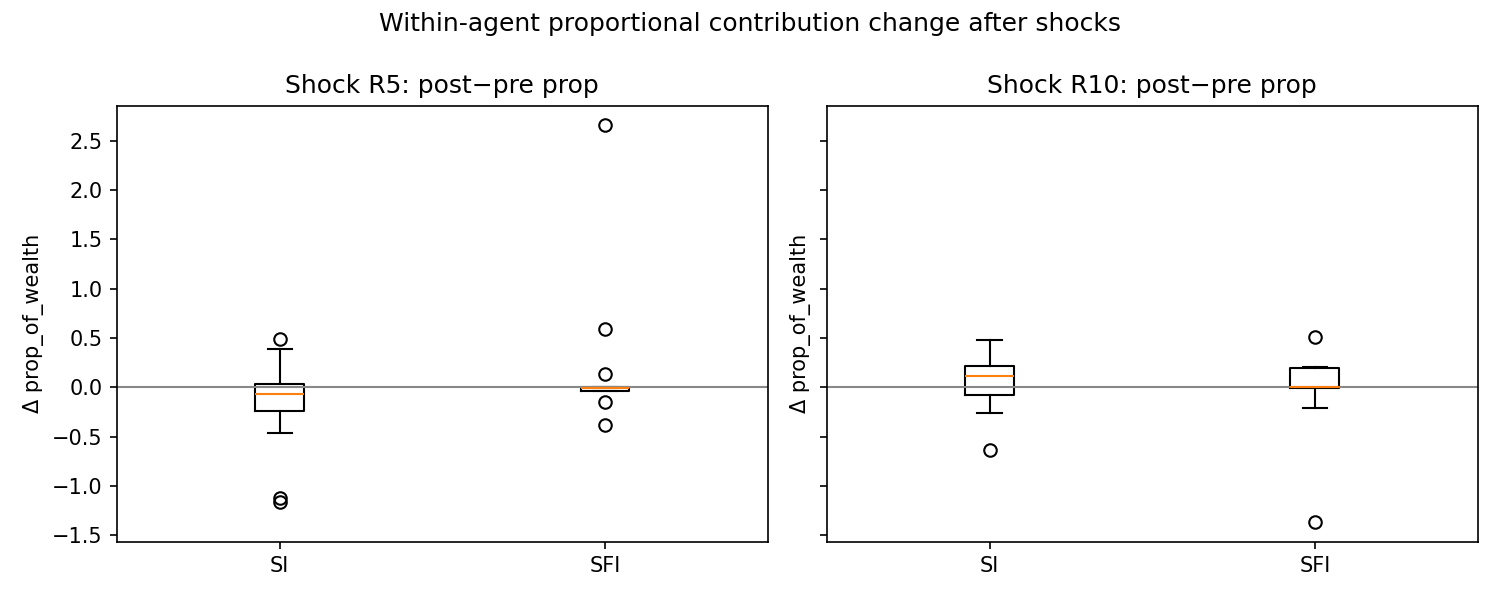
\includegraphics[width=\linewidth]{figures/shock_delta_boxplot.png}
\caption{Within-agent changes in contribution intensity around climatic shocks.
The first shock coincides with a sharp SI decline.
The second shock shows mixed signs.}
\label{fig:shock_box}
\end{figure}

Democracy sessions occur at both shock rounds.
Shock effects are therefore not cleanly separable from rule updates.
We treat shock panels as environmental context for social-pressure results.

\subsection{Wealth, fund coverage, and inequality}

Figure~\ref{fig:wealth_gap} tracks the developed--developing wealth gap.
The gap widens from $4.56\times10^{6}$ in round~1 to $2.15\times10^{8}$ in round~30.
Absolute Stage-1 contribution means differ by roughly two orders of magnitude across institutions because wealth stocks differ.
Intensity means remain close.
Scale inequality and behavioral intensity are distinct objects.

\begin{figure}[t]
\centering
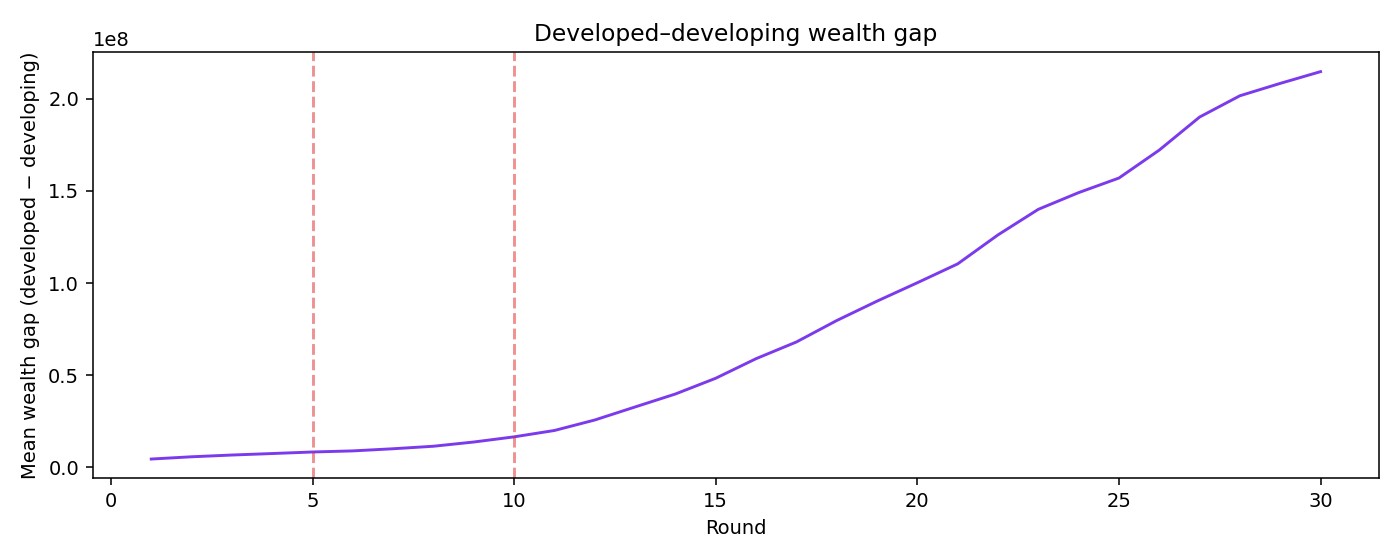
\includegraphics[width=\linewidth]{figures/wealth_gap_developed_developing.png}
\caption{Developed-minus-developing aggregate wealth over rounds.
The gap widens despite dual-use deposits and shock payouts.}
\label{fig:wealth_gap}
\end{figure}

Figure~\ref{fig:ldf} shows loss-and-damage pool dynamics.
The pool accumulates far beyond cumulative payouts.
Shock coverage equals 0.768 in both shock rounds.
Cumulative payouts are on the order of $8.5\times10^{5}$ currency units.
Terminal pool balance is orders of magnitude larger.
Coverage without equalization is the descriptive summary.
Fund language appears in only about 1.8\% of contribution rationales.
Agents rarely narrate dual-use deposits as the binding motive.

\begin{figure}[t]
\centering
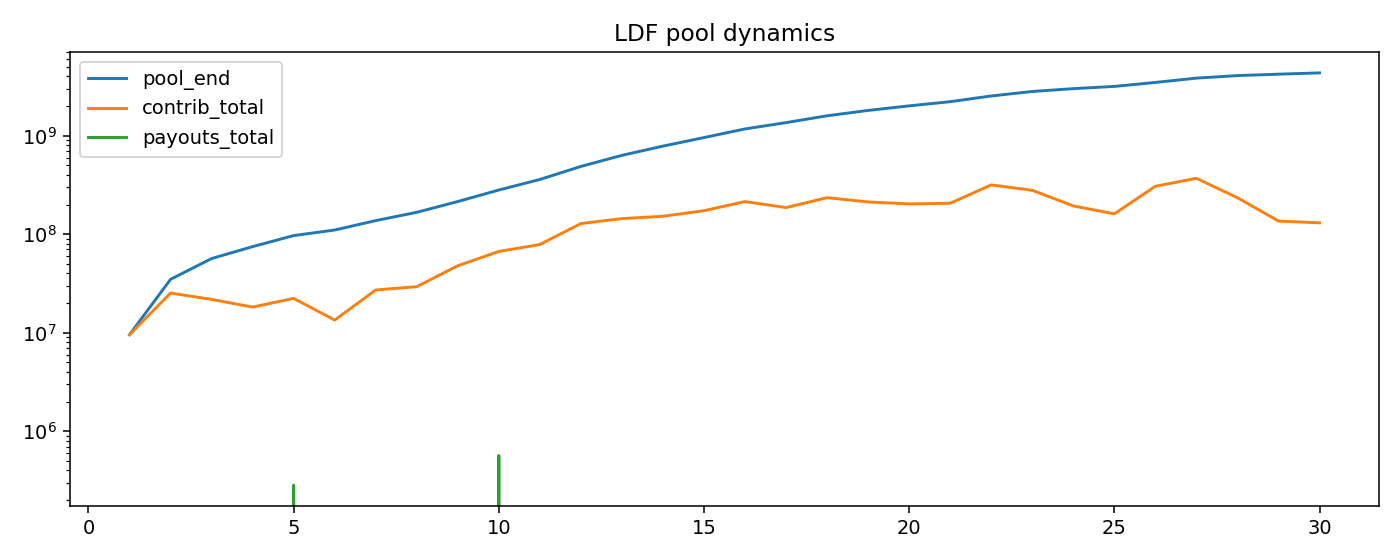
\includegraphics[width=\linewidth]{figures/ldf_pool_dynamics.png}
\caption{Loss-and-damage pool balance versus payout events.
Collection and growth dominate disbursement.}
\label{fig:ldf}
\end{figure}

Figure~\ref{fig:gini} plots wealth Gini against a cooperation-rate summary.
Wealth Gini falls from 0.709 in round~1 to 0.556 mid-run, then rises to 0.653 by round~30.
The U-shape indicates temporary compression followed by renewed dispersion.
Inequality statistics reinforce that social-pressure findings occur inside a diverging wealth path.

\begin{figure}[t]
\centering
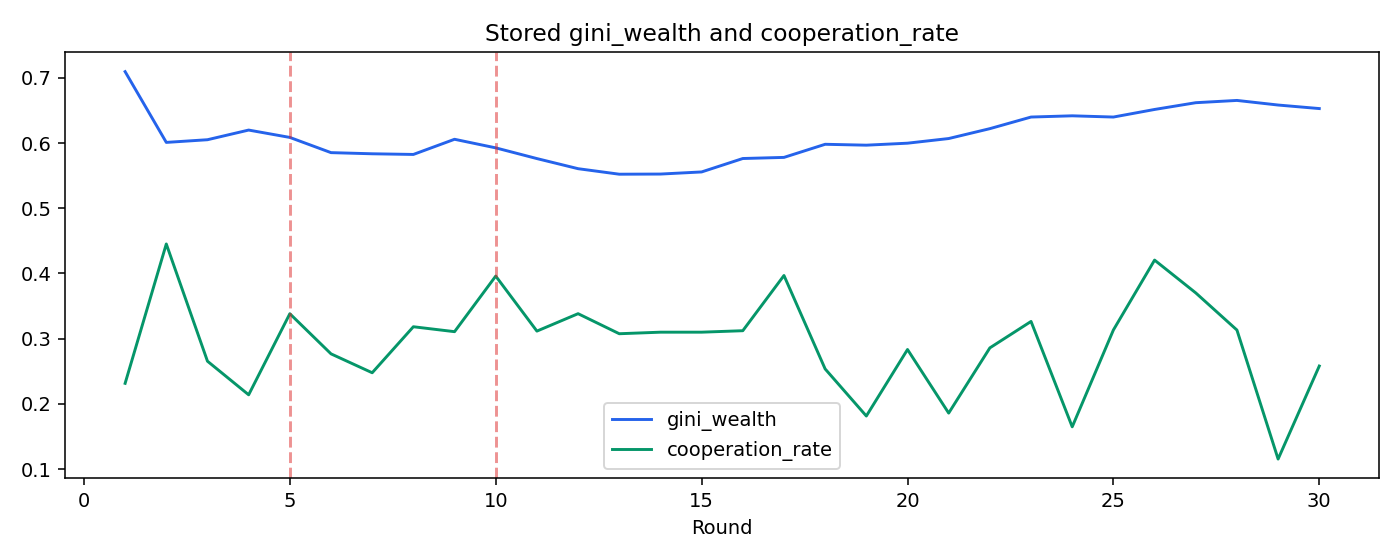
\includegraphics[width=\linewidth]{figures/gini_wealth_cooperation_rate.png}
\caption{Wealth Gini and cooperation-rate summary across rounds.
Inequality compresses mid-run then widens again.}
\label{fig:gini}
\end{figure}

\subsection{Sanctions, rewards, and enforcement burden}

Figure~\ref{fig:sanctions} shows punishment and reward timelines inside SI.
Sanction activity varies across rounds rather than locking into a stable high-punishment regime.
Figure~\ref{fig:enforcement} summarizes enforcement burden.
Correlation between contribution intensity and Stage-2 tokens spent is about 0.14.
Top-quartile intensity agents account for roughly 35\% of enforcement tokens.
Enforcement is costly and uneven.
It does not substitute for the gossip channel in SFI, where Stage-2 is unavailable.

\begin{figure}[t]
\centering
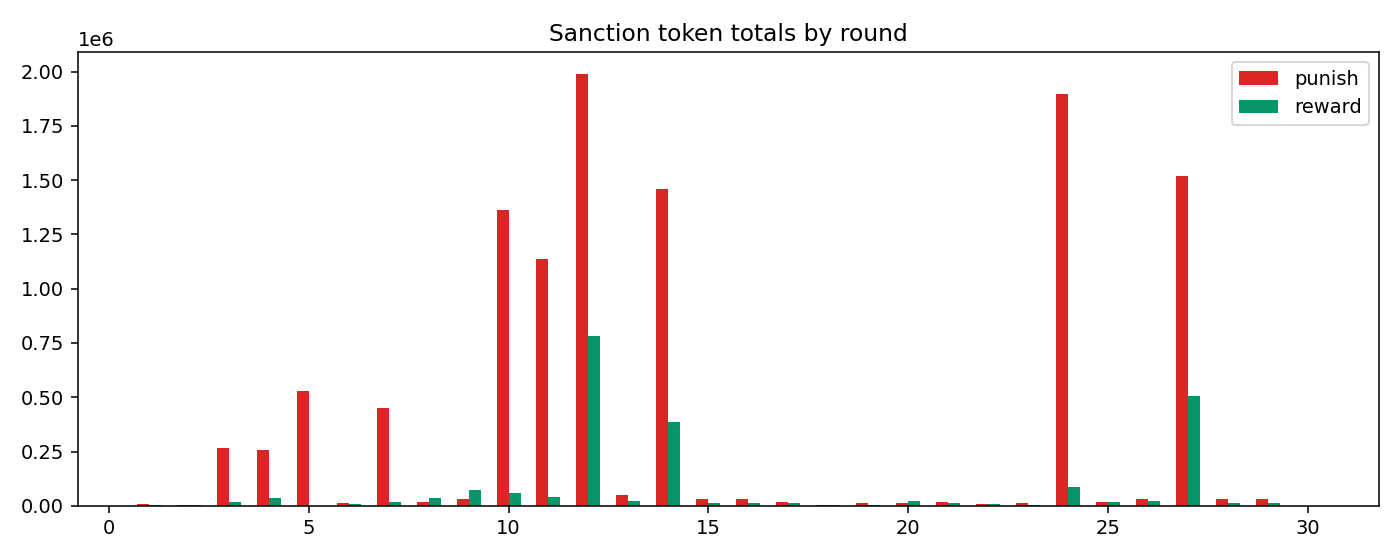
\includegraphics[width=\linewidth]{figures/sanction_punish_reward_timeline.png}
\caption{Aggregate punishment and reward allocations over rounds in the enforcing institution.}
\label{fig:sanctions}
\end{figure}

\begin{figure}[t]
\centering
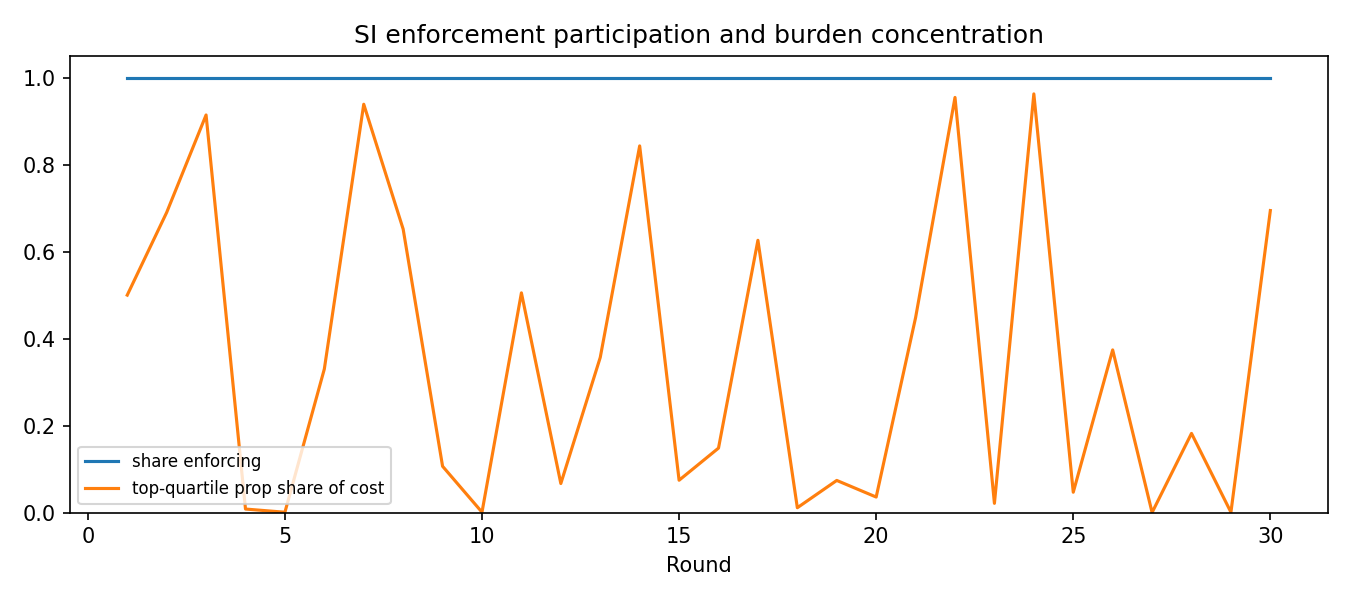
\includegraphics[width=\linewidth]{figures/enforcement_burden.png}
\caption{Enforcement spending relative to contribution intensity.
Higher-intensity agents bear a sizable share of Stage-2 tokens.}
\label{fig:enforcement}
\end{figure}

\subsection{Democratic adaptation as institutional backdrop}

Figure~\ref{fig:democracy} displays adopted rules over constitutional sessions.
Six sessions yield fourteen proposals and six adoptions.
Adopted changes raise subsidy fraction, raise loss-and-damage equity weight, and raise damage weight in payouts.
Punishment-weakening proposals appear twice and fail both times.
Proposers are split across institutions (eight SI, six SFI).
Mean proposer intensity (0.36) exceeds population mean intensity (0.29).
Vote alignment with proposer institution is near base rate.

\begin{figure}[t]
\centering
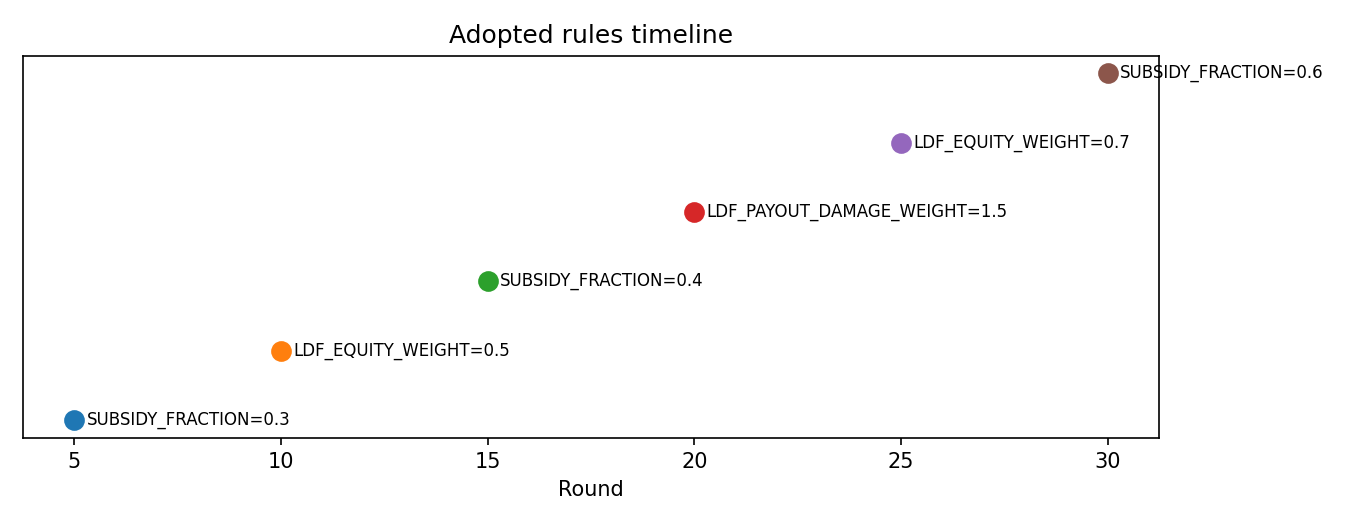
\includegraphics[width=\linewidth]{figures/adopted_rules_timeline.png}
\caption{Timeline of democratically adopted parameter changes.
The path favors higher subsidies and stronger loss-and-damage equity settings.}
\label{fig:democracy}
\end{figure}

Democracy therefore drifts toward carrots and equity weights while preserving punishment strength.
That path is politically informative.
It is not the primary reputation claim.
It shows that agents can revise fiscal parameters while still reducing intensity after social stigma.

\subsection{Norm emergence versus cooperation levels}

Late-round dispersion remains large.
Late interquartile range of intensity is 0.178 versus 0.238 early.
Near-zero agents number 5 of 26.
High-intensity agents (mean at least 0.25) number 13 of 26.
Conditional-cooperation correlations with peer history are weak (about 0.05 in SI and $-0.09$ in SFI over the full path).
Fairness and reciprocity tokens are rare in shared contribution language.
The synthesis verdict is limited or mixed norm emergence alongside moderately positive average transfers.
Positive means do not imply internalized contribution norms.
The reputation result sits inside that distinction.
Social marks do not convert into a repair norm in this run.
